% !TEX program = pdflatex
\documentclass[11pt,a4paper]{article}

% -------------------------
% Language and fonts
% -------------------------
\usepackage[utf8]{inputenc}
\usepackage[T1]{fontenc}
\usepackage[english]{babel}
\usepackage{lmodern}

% -------------------------
% Layout
% -------------------------
\usepackage[a4paper,margin=2.5cm]{geometry}
\usepackage{setspace}
\setstretch{1.12}
\usepackage{microtype}

% -------------------------
% Utilities
% -------------------------
\usepackage{graphicx}
\usepackage{booktabs}
\usepackage{enumitem}
\usepackage{hyperref}
\hypersetup{
  colorlinks=true,
  linkcolor=blue,
  urlcolor=blue,
  citecolor=blue
}

% -------------------------
% TikZ (flowchart)
% -------------------------
\usepackage{tikz}
\usetikzlibrary{arrows.meta,positioning,shapes.geometric}

% -------------------------
% Title
% -------------------------
\title{\textbf{Automatic Documentation Methodology (C + Python)\\
with Sphinx, Doxygen, Breathe and Read the Docs}}
\author{Project: SDR Sensor \\
Team: \textit{(Fill names)}}
\date{\today}

\begin{document}
\maketitle

\begin{abstract}
This document describes, in a conceptual way, the methodology used to unify the automatic documentation of a hybrid repository (C and Python code) into a single publishable site. The approach integrates: (i) extraction of documentation from Python docstrings, (ii) extraction of documentation from C comments and signatures, and (iii) final assembly in a Sphinx-generated website, compatible with Read the Docs deployment.
\end{abstract}

\section{Context and problem}
The project worked on two documentation lines developed in separate copies of the same repository:

\begin{itemize}[leftmargin=*,itemsep=2pt]
  \item \textbf{Copy A (C-focused):} aimed at documenting \texttt{.c/.h} files using Doxygen and its structured output.
  \item \textbf{Copy B (Python-focused):} aimed at documenting \texttt{.py} modules using autodocumentation (docstrings) rendered by Sphinx.
\end{itemize}

The problem was to \textbf{merge both approaches} to obtain a \textbf{single documentation site} (same navigation tree, same visual theme, same configuration) where both the C API and the Python API coexist.

\section{Goal}
\begin{itemize}[leftmargin=*,itemsep=2pt]
  \item Centralize documentation under a single \texttt{docs/} tree with one Sphinx configuration.
  \item Preserve automatic generation for both languages:
  \begin{itemize}[leftmargin=*,itemsep=2pt]
    \item \textbf{Python:} from docstrings and module/class/function signatures.
    \item \textbf{C:} from Doxygen (structured output) embedded into Sphinx through Breathe.
  \end{itemize}
  \item Enable reproducible builds locally and on a documentation hosting service (e.g., Read the Docs).
\end{itemize}

\section{Solution architecture}
The unification is based on \textbf{clearly separating sources of truth} and \textbf{connecting both worlds through a stable integration point}:

\begin{itemize}[leftmargin=*,itemsep=2pt]
  \item \textbf{Python source of truth:} docstrings (Google/NumPy style) + Sphinx code introspection.
  \item \textbf{C source of truth:} Doxygen-style comments/tags in \texttt{.h/.c}.
  \item \textbf{Integration:} Doxygen produces a \textit{structured representation} and Breathe allows Sphinx to consume and display it within the final site.
\end{itemize}

\subsection{Components and responsibilities}
\begin{table}[h]
\centering
\begin{tabular}{@{}p{3.3cm}p{10.5cm}@{}}
\toprule
\textbf{Component} & \textbf{Role in the pipeline} \\
\midrule
Sphinx & Site orchestrator: processes \texttt{.rst}, resolves references, and generates final HTML. \\
Autodoc / Napoleon & Extract and format documentation from Python docstrings (classes, functions, attributes). \\
Doxygen & Analyzes C/C++ and produces structured output from comments/signatures (ideally XML). \\
Breathe & Bridges Doxygen output into Sphinx; provides directives to “include” C entities in \texttt{.rst} pages. \\
Visual theme (e.g., Furo) & Defines website look and feel (navigation, typography, sidebar, etc.). \\
Optional extensions (e.g., Mermaid) & Add diagrams and enriched content if the project requires it. \\
\bottomrule
\end{tabular}
\end{table}

\section{Unified workflow (step-by-step, conceptual)}
The logical workflow is organized in phases, prioritizing reproducibility and traceability:

\subsection{Phase 1: Documentation structure normalization}
\begin{itemize}[leftmargin=*,itemsep=2pt]
  \item Define a \textbf{single documentation directory} (e.g., \texttt{docs/}).
  \item Under \texttt{docs/source/}, organize content into coherent sections:
  \begin{itemize}[leftmargin=*,itemsep=2pt]
    \item System chapters (architecture, installation, operation).
    \item Python API.
    \item C API (e.g., under \texttt{c\_api/} with its own \texttt{index.rst}).
  \end{itemize}
  \item Define a \textbf{main toctree} that links both APIs and all remaining chapters.
\end{itemize}

\subsection{Phase 2: Structured artifact generation for C}
\begin{itemize}[leftmargin=*,itemsep=2pt]
  \item Configure Doxygen to \textbf{traverse the real folders} containing the C code to document.
  \item Generate Doxygen output in a structured format suitable for integration (typically XML).
  \item Validate that the output includes an entry index (anchor point) and entity artifacts (structs, functions, defines, typedefs).
\end{itemize}

\subsection{Phase 3: C integration into Sphinx}
\begin{itemize}[leftmargin=*,itemsep=2pt]
  \item Configure Sphinx to know the path to the Doxygen output.
  \item Enable Breathe to expose directives that \textbf{render C entities} inside \texttt{.rst} pages.
  \item Build \texttt{.rst} pages that act as “bridges” between site navigation and C objects.
\end{itemize}

\subsection{Phase 4: Python automatic documentation}
\begin{itemize}[leftmargin=*,itemsep=2pt]
  \item Sphinx (with autodoc and napoleon) imports Python code and \textbf{extracts docstrings}.
  \item The final site publishes the Python API consistently (modules, classes, functions).
  \item Difficult external dependencies are handled via isolation techniques (so builds do not fail due to missing heavy libraries).
\end{itemize}

\subsection{Phase 5: Final assembly, validation, and publication}
\begin{itemize}[leftmargin=*,itemsep=2pt]
  \item Sphinx generates the final HTML by integrating global navigation with both APIs.
  \item Review typical warnings: ambiguous references, duplicates, missing entities, wrong paths.
  \item Prepare deployment on a reproducible hosting environment (e.g., Read the Docs), ensuring dependencies are installed and the pipeline runs end-to-end.
\end{itemize}

\section{Pipeline flowchart}
\begin{figure}[h]
\centering
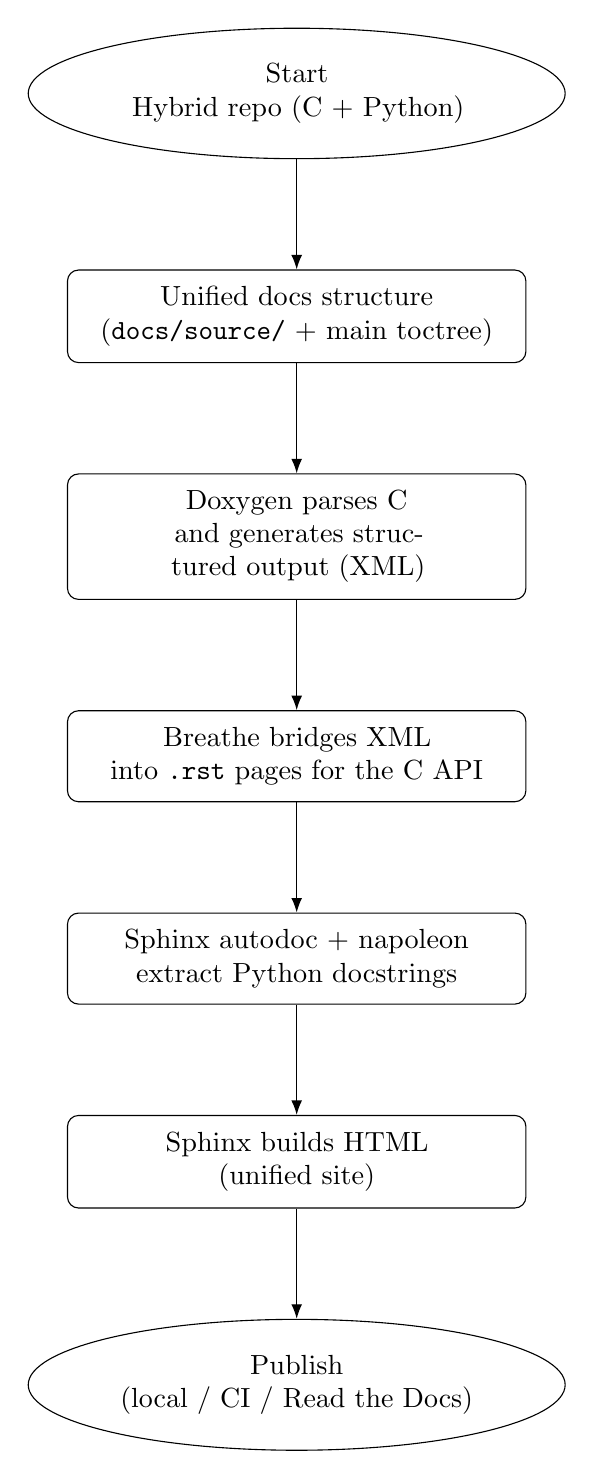
\begin{tikzpicture}[
  node distance=14mm,
  box/.style={rectangle, rounded corners, draw, align=center, inner sep=6pt, text width=5.4cm},
  startstop/.style={ellipse, draw, align=center, inner sep=6pt, text width=4.4cm},
  arrow/.style={-{Latex}, line width=0.5pt}
]
\node[startstop] (start) {Start\\Hybrid repo (C + Python)};
\node[box, below=of start] (structure) {Unified docs structure\\(\texttt{docs/source/} + main toctree)};
\node[box, below=of structure] (doxygen) {Doxygen parses C\\and generates structured output (XML)};
\node[box, below=of doxygen] (breathe) {Breathe bridges XML\\into \texttt{.rst} pages for the C API};
\node[box, below=of breathe] (autodoc) {Sphinx autodoc + napoleon\\extract Python docstrings};
\node[box, below=of autodoc] (build) {Sphinx builds HTML\\(unified site)};
\node[startstop, below=of build] (deploy) {Publish\\(local / CI / Read the Docs)};

\draw[arrow] (start) -- (structure);
\draw[arrow] (structure) -- (doxygen);
\draw[arrow] (doxygen) -- (breathe);
\draw[arrow] (breathe) -- (autodoc);
\draw[arrow] (autodoc) -- (build);
\draw[arrow] (build) -- (deploy);
\end{tikzpicture}
\caption{Conceptual pipeline for automatic documentation in a hybrid repository.}
\end{figure}

\section{Verification strategy (conceptual ``checks'')}
To ensure automation actually documents what it should, verification is based on observable evidence:

\begin{itemize}[leftmargin=*,itemsep=2pt]
  \item \textbf{Input verification:} confirm target C/Python folders exist and contain expected files.
  \item \textbf{Artifact verification:} ensure the C structured output contains an entry index and enough objects (structs/functions) to be referenced.
  \item \textbf{Reference resolution verification:} detect ambiguities when the same name is published from different paths/domains.
  \item \textbf{Site consistency verification:} ensure navigation links to the new sections (C API) and the final render does not leave orphan pages.
\end{itemize}

\section{Common risks and how they are handled (conceptual)}
\begin{itemize}[leftmargin=*,itemsep=2pt]
  \item \textbf{Unknown directives:} typically means the responsible extension is not enabled (e.g., the layer that integrates Doxygen with Sphinx).
  \item \textbf{C entities ``not found'':} often due to incomplete structured output (wrong input paths or missing output generation).
  \item \textbf{Duplicate/ambiguous references:} occur when the same object is documented from multiple paths or indices see equivalent definitions.
  \item \textbf{Non-compatible docstring syntax:} some markup may not be supported; describing attributes/fields with supported structured text is safer than using non-standard directives.
\end{itemize}

\section{Conclusions}
The methodology successfully merged two complementary approaches:
\begin{itemize}[leftmargin=*,itemsep=2pt]
  \item \textbf{Native Python documentation} based on docstrings and introspection.
  \item \textbf{Structured C documentation} based on static analysis with Doxygen.
\end{itemize}
The result is a single, extensible, publishable pipeline where documentation stays close to the code, reducing manual effort and improving long-term consistency.

\section*{References (methodology and tools)}
\begin{thebibliography}{9}

\bibitem{sphinx-autodoc}
Sphinx Documentation. \textit{Automatic documentation generation (autodoc)}.\\
\url{https://www.sphinx-doc.org/en/master/usage/extensions/autodoc.html}

\bibitem{sphinx-napoleon}
Sphinx Documentation. \textit{Napoleon (Google/NumPy docstrings)}.\\
\url{https://www.sphinx-doc.org/en/master/usage/extensions/napoleon.html}

\bibitem{doxygen-config}
Doxygen Manual. \textit{Configuration options (incl.\ OUTPUT\_DIRECTORY, GENERATE\_XML, XML\_OUTPUT)}.\\
\url{https://www.doxygen.nl/manual/config.html}

\bibitem{breathe}
Breathe Documentation. \textit{Breathe: reStructuredText directives for Doxygen output}.\\
\url{https://breathe.readthedocs.io/en/latest/directives.html}

\bibitem{rtd-sphinx}
Read the Docs Documentation. \textit{Deploying Sphinx on Read the Docs}.\\
\url{https://docs.readthedocs.com/platform/stable/intro/sphinx.html}

\bibitem{mermaid}
PyPI. \textit{sphinxcontrib-mermaid: Mermaid diagrams for Sphinx}.\\
\url{https://pypi.org/project/sphinxcontrib-mermaid/}

\bibitem{furo}
Furo Theme Documentation. \textit{Furo: Sphinx documentation theme}.\\
\url{https://pradyunsg.me/furo/}

\end{thebibliography}

\end{document}
